\subsection{从 GCN 编码器到 GAE 与点对表示}
GCN 是邻域传播的\emph{编码器}，典型层可写为
\begin{equation}
H^{(\ell+1)}=\sigma\!\left(\widetilde D^{-1/2}\widetilde A\widetilde D^{-1/2}H^{(\ell)}W^{(\ell)}\right),\quad H^{(0)}=X,
\end{equation}
其中 $\widetilde A=A+I$\cite{kipf2017gcn}。GAE 是\emph{编码器、链路解码器和重构目标}构成的框架；常用 GCN 编码后，以 $\sigma(h_u^\top h_v)$ 预测边，VGAE 另引入潜变量分布与变分约束\cite{kipf2016vgae}。因此使用 GCN 的链路预测模型通常也可视为 GAE 类模型，二者不是互斥模型名称。本文三个模型主要区别在于如何构造和解码待预测点对的信息。

SEAL 通过目标点对的包围子图和节点标号构造链路表示\cite{zhang2018seal}；ELPH/BUDDY 采用子图草图、邻域结构统计与预计算，提高点对结构建模的效率\cite{chamberlain2023buddy}。NCNC 则在先编码节点之后进行共同邻域聚合，LPFormer 使用对不同点对自适应的注意力上下文。Refined-GAE 保留较简洁的编码解码框架，强调输入表示、训练配方与解码器设计。选择三者有助于比较显式局部结构、学习式点对上下文与强 GAE 基线。

作为本仓库的研究背景，SGDiff 将链路判断转化为包围子图的类别条件似然估计\cite{li2025sgdiff}，涉及连续 DDPM 与离散状态扩散思想\cite{ho2020ddpm,austin2021d3pm}。本报告没有对 SGDiff 重新运行同一批图，故不把历史 SGDiff 数值加入模型排名；这里的相关工作介绍只解释比较动机。

\subsection{NCNC：神经共同邻居及缺失关系补全}
\textbf{论文与思路。}Wang、Yang 与 Zhang 的 NCNC发表于 ICLR 2024\cite{wang2024ncnc}。NCN 先用消息传递得到节点状态，再根据候选点对 $(u,v)$ 的共同邻居聚合其状态。区别于单纯统计共同邻居个数，它能同时编码共同邻居携带的属性与传播信息。NCNC 进一步处理图不完整导致的共同邻居缺失：对仅与一端连接的节点，估计另一条关系存在的概率，并用校准后的权重加入聚合。
\begin{equation}
 c_{uv}=\sum_{w\in N(u)\cap N(v)}h_w,
 \quad \widetilde c_{uv}=c_{uv}
 +\sum_{w\in N(u)\setminus N(v)}\omega_{vw}h_w
 +\sum_{w\in N(v)\setminus N(u)}\omega_{uw}h_w .
\end{equation}
该式是本次实现的概念表达；$\omega$ 由低深度预测器与作者的概率校准产生，不意味着在输入图中永久添加所有预测边。最终预测器结合端点 Hadamard 乘积和共同邻域分支。本次一次补全的候选概率预测沿用作者 \code{no_grad} 路径，并未把补全过程改成端到端图生成。
\Fig{ncnc_evaluated_architecture.pdf}{1.0}{本次 NCNC 适配器的计算流程，由作者代码及实际配置整理绘制。绿色部分为显式点对结构建模；noCN 仍保留 GCN 的结构传播。}{fig:ncnc}
\begin{figure}[htbp]\centering
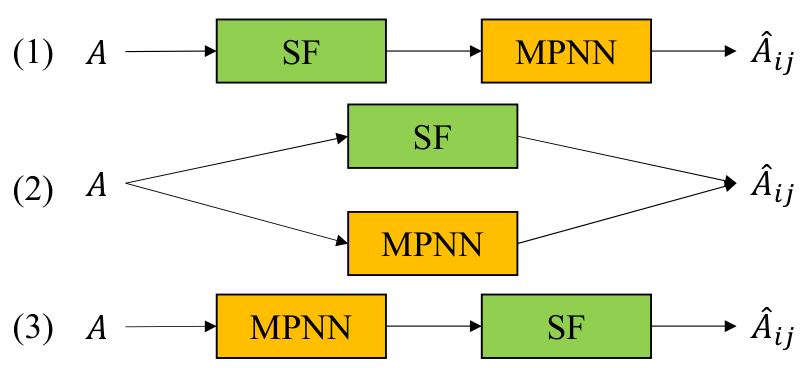
\includegraphics[width=.55\linewidth]{figures/ncnc_original_fig2.png}
\caption{NCNC 原论文第2页 Figure 2 的示意图区域摘录\cite{wang2024ncnc}：不同的结构特征与消息传递组合顺序。原图版权归原作者，保留原标签，未包含原文图注。该图描述架构类别，不是本次完整训练流程。}\label{fig:ncnc-original}
\end{figure}
\textbf{本次配置与问题。}调用固定作者的 GCN 与 \code{IncompleteCN1Predictor}；三个数据集均使用256维、一层编码、一次补全，不截断补全候选。比较完整模型与 noCNC、noCN，检验收益是否由补全或显式共同邻域产生。随机删边会使一条共同邻域证据依赖的两条边同时保留的概率下降，这是机制假设，实际贡献仍由配对消融判断。

\subsection{LPFormer：点对注意力与 PPR 上下文}
\textbf{论文与思路。}Shomer 等人的 LPFormer 发表于 KDD 2024\cite{shomer2024lpformer}。它为每个候选点对形成不同的上下文：先编码节点，再利用个性化 PageRank（PPR）筛选共同邻居、单侧邻居和较远节点，最后按节点状态及点对位置编码进行注意力聚合。PPR 的局部推送近似与经典局部图划分方法相关\cite{andersen2006ppr}。
\begin{equation}
 s_{uv}=\sum_{w\in\widehat N(u,v)}\alpha_{uvw}\,V\!\left(h_w,\mathrm{PE}(u,v,w)\right),
 \qquad \sum_{w\in\widehat N(u,v)}\alpha_{uvw}=1.
\end{equation}
这是省略多头和投影细节的示意式。作者最终将点对聚合、端点交互和类别计数送入预测头。PPR 在这里有两种作用：\emph{决定候选集合}与\emph{提供位置编码数值}，因此只将位置编码置零并不等于删除全部 PPR 信息。
\Fig{lpformer_evaluated_architecture.pdf}{1.0}{本次 LPFormer 适配器流程的重新绘制。结构攻击通过 GCN、PPR 候选、位置编码和计数共同影响输出；本报告未将这些影响拆成独立因果路径。}{fig:lpformer}
\begin{figure}[htbp]\centering
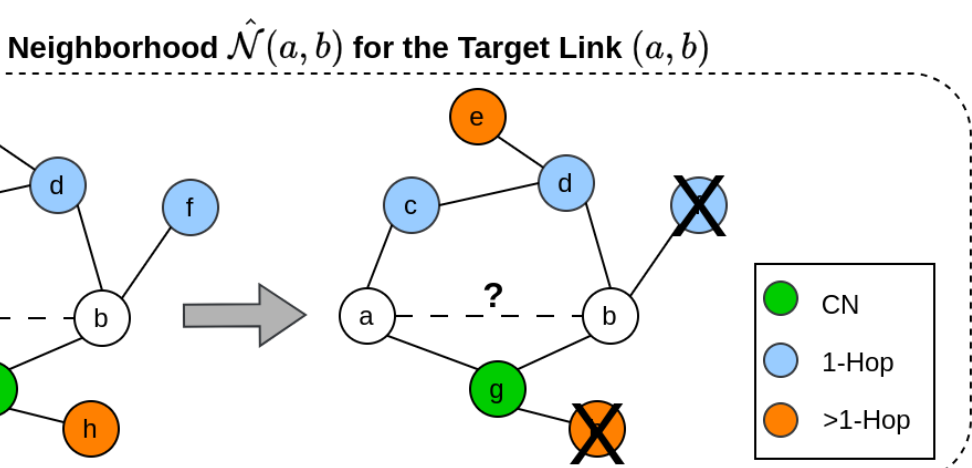
\includegraphics[width=.55\linewidth]{figures/lpformer_original_fig2_panel2.png}
\caption{LPFormer 原论文第4页 Figure 2 的第2面板局部摘录\cite{shomer2024lpformer}，展示目标点对的候选邻域筛选。原图版权归原作者；仅保留该面板，完整实际流程见图\ref{fig:lpformer}。}\label{fig:lp-original}
\end{figure}
\textbf{本次配置与问题。}调用作者 \code{LinkTransformer} 与 MLP 预测头，一层 GCN、一层点对注意力、一个注意力头；Cora/Citeseer/PubMed 的维数为128/256/128。Uniform 将注意力向量置零并冻结，候选内权重均匀，保留值投影；noPE 将位置编码输出置零，保留候选与计数。每张不同攻击图均重新计算 PPR，避免在新图上错误复用旧结构编码。训练时沿用作者全训练图 PPR，局部传播和邻域则移除当前批次目标边，因此 PPR 仍可能携带批次训练目标信息。

\subsection{Refined-GAE：较简洁传播与强解码器}
\textbf{论文与思路。}Ma 等人的 \emph{Reconsidering the Performance of GAE in Link Prediction} 发表于 CIKM 2025\cite{ma2025refined}。本文以作者代码库名 Refined-GAE 标识该工作，避免与原始 GAE 混淆。该工作强调合理选择初始表示、传播和预测器，而不把模型复杂度本身作为提升的证据。其线性邻域聚合与深度加权的思路可与 LightGCN 对照\cite{he2020lightgcn}；但作者代码中名为 \code{LightGCN} 的模块并非推荐任务原始 LightGCN 的逐行复制。

\textbf{本次实际实现。}使用已有节点属性，不新增每节点可学习 ID 嵌入，因此没有在本实验中直接检验无属性图上的正交 ID 初始化论点。首步完成归一化传播与特征投影，后续步骤共享无权重传播算子；步间使用 LayerNorm 与 dropout，各深度输出以可学习 softmax 系数加权。这里 LayerNorm 是逐节点隐藏表示归一化\cite{ba2016layernorm}，不同于输入列标准化和邻接度归一化。
\begin{equation}
 z_u=\sum_{\ell=1}^L\mathrm{softmax}(a)_\ell h_u^{(\ell)},
 \qquad f(u,v)=\mathrm{MLP}(z_u\odot z_v).
\end{equation}
Cora/Citeseer 使用4步传播和1024维；PubMed 使用2步和512维，深度参数初始为 $[1,0.5]$，随后经 softmax 并训练，不能称为固定指数权重。Cora 解码器为4层 SiLU 残差 MLP，Citeseer 为2层 ReLU MLP，PubMed 为2层 GELU MLP。
\Fig{refined_evaluated_architecture.pdf}{1.0}{本次 Refined-GAE 适配器的实际路径示意。noLN 仅删除编码器/解码器 LayerNorm；Dot 用作者点积预测器替代完整预测头，两者均独立重训。}{fig:refined}
\begin{figure}[htbp]\centering
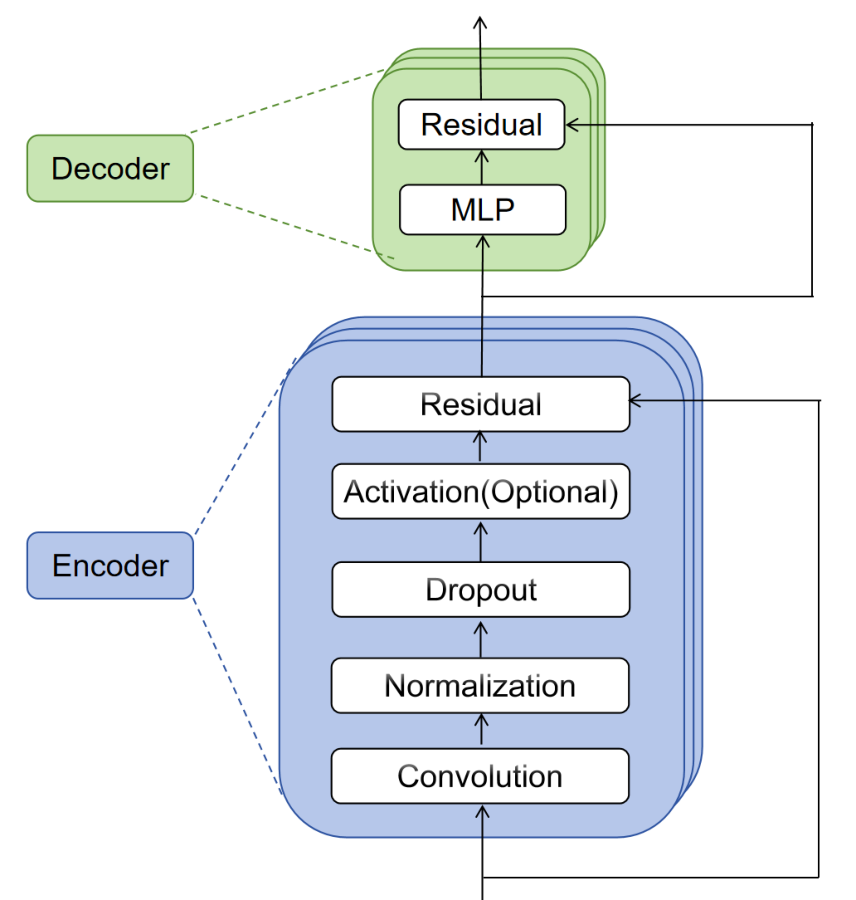
\includegraphics[height=6cm]{figures/refined_original_fig2.png}
\caption{Refined-GAE 论文 arXiv v4 第4页 Figure 2 的原示意图区域摘录\cite{ma2025refined}。这是论文对典型 GAE 编码器/解码器模块的概览，包含可选项；不是本次每个数据集具体启用项的列表。原图版权归原作者。}\label{fig:refined-original}
\end{figure}
\textbf{本次关注。}noLN 保留 dropout 以及输入与邻接归一化，用于检验网络内 LayerNorm；Dot 保留编码器架构后重新训练，用于检验完整非线性解码设计。后者同时改变参数量、非线性、正则化和训练轨迹，不能解释为在冻结编码器上只替换打分公式。

\subsection{源码版本与图像出处}
以下源码均固定提交并校验逐文件 SHA-256。报告新增图为本次独立绘制，三个原图局部的页码、裁剪范围与源 PDF 指纹保存在 \code{figure_sources.json}；Refined-GAE 引用正式2025版本，并选取对应 arXiv v4 示意图，不使用早期预印本不同的图号解释当前图。
\begin{itemize}
\item \href{https://github.com/GraphPKU/NeuralCommonNeighbor/tree/11d597013750da17ce7468e344bec756a7af39a4}{NCNC 作者代码}：\code{11d597013750da17ce7468e344bec756a7af39a4}。
\item \href{https://github.com/HarryShomer/LPFormer/tree/3ca80aba3bd1ba4903ec5c042608e4a034110c9f}{LPFormer 作者代码}：\code{3ca80aba3bd1ba4903ec5c042608e4a034110c9f}。
\item \href{https://github.com/GraphPKU/Refined-GAE/tree/5bcf00ee42134a31995bbc7bcc5359810aa99b6c}{Refined-GAE 作者代码}：\code{5bcf00ee42134a31995bbc7bcc5359810aa99b6c}。
\end{itemize}
